\section{Experimentacion General}
En esta secci\'on analizaremos la calidad de las heuristicas mediante la comparaci\'on y analisis estadistico de las soluciones, asi tambien el tiempo insumido en obtener dichas soluciones, para diferentes grupos de instancias de grafos generados al azar.

\subsection{Generacion de conjuntos de grafos aleatorios}

\subsubsection{Generador de grafos aleatorios}
El generador aleatorio de grafos es un binario aparte de los algoritmos, que recibe como parametros
\begin{itemize}
\item cantidad de nodos
\item cantidad de aristas
\item peso minimo $w_1$
\item peso maximo $w_1$
\item peso minimo $w_2$
\item peso maximo $w_2$
\item limite $w_1$
\end{itemize}
y devuelve por salida estandar una instancia del problema tal como esta especificado el formato de entrada en el enunciado de este TP.\\
\textbf{Nota: }Los generadores de numeros aleatorios de este generador de grafos tienen distribucion uniforme(Usan random de C++11).

\vspace{1cm}

La generaci\'on del grafo se realiza de la siguiente manera: 
Sean n=\{cantidad de nodos del grafo\} y m=\{cantidad de aristas\}, se inicializa un vector $aristas =  <(0, 1), ..., (0, n-1), (1, 2), ..., (1, n-1), ..., (n - 2, n-1)>$ conteniendo todas las aristas posibles en el grafo(notar que como no es digrafo, no se repiten aristas simetricas, ni tampoco de asignan self-loops).

\vspace{1cm}

Luego se mezcla aleatoriamente este vector usando el \texttt{Algoritmo de Shuffle de Knuth o Fisher Yates Shuffle} y se imprime la cabecera del grafo a la salida estandar conteniendo los nodos origen, destino y el parametro k generados como numeros aleatorios uniformes. Ahora basta tomar la cantidad m de aristas requeridas por par\'ametro y serializar la salida linea por linea, nuevamente generando numeros aleatorios con distribucion uniforme sobre los rangos de pesos $w_1$ y $w_2$ pasados por par\'ametro.

\subsubsection{Script generador de conjuntos de grafos}
Se realizo un script el cual genera conjuntos de grafos usando el generador de la seccion anterior, basicamente, se setean dos rangos, de cantidad de nodos y cantidad de aristas, y los parametros fijos como limite $w_1$, limites de los pesos, etc. El script genera iterativamente el conjunto de grafos llamando repetidamente al generador, notemos que podemos(y es lo que hicimos en los experimentos), poner la cantidad de aristas en funcion de la cantidad de nodos y de esta forma poder determinar la densidad de los conjuntos de grafos generados.

\subsection{Scripts de optimalidad - Calculo de puntajes y estadisticas}
Se realizaron diversos scripts para automatizar el analisis de optimalidad y performance, vamos a analizar el script de optimalidad que se ejecuto para obtener los resultados de esta secci\'on.\\
Se trata de un script en bash que para cada instancia del conjunto de grafos generados aleatoriamente, ejecuta los 4 algoritmos (exacta, golosa, busqueda local, grasp) y va realizando calculos estadisticos de los resultados obtenidos, tanto de la solucion como del tiempo consumido para obtenerla.
Los analisis estadisticos que se realizan son:\\
\begin{itemize}
	\item Tiempo promedio microsegundos consumido por el algoritmo
	\item Porcentaje de veces que la heuristica da la solucion optima
	\item Desviacion estandar de veces que la heuristica da la sol. optima
	\item Lejan\'ia promedio de la solucion obtenida a la solucion optima
	\item Desviacion estandar de la lejan\'ia de las soluciones entre la obtenida y la optima
	\item Minima y maxima lejan\'ia obtenida en este conjunto de instancias
\end{itemize}

\textbf{Nota: }La lejan\'ia entre 2 soluciones se mide haciendo el siguiente calculo: 
$ 100 *(\frac{solucionHeuristica}{solucionOptima} - 1)  $ que indica en porcentaje cual es el ratio de distancia entre los dos valores del cociente.\\
\textbf{Nota: } Los calculos estadisticos (promedio y desviacion estandar) se realizan sobre la lista de resultados obtenida de la ejecucion secuencial y el calculo de la lejania mencionado aqui arriba para cada uno de los algoritmos(exacto y heuristica) sobre cada instancia del conjunto de pruebas.

Podemos considerar una especie de puntuacion asignada a cada heuristica viendo el porcentaje de optimalidad y tambien podemos analizar, que cuando no da la solucion optima, la lejania a la optima, con cierta dispersion sea adecuada, segun el problema y el las necesidades del contexto donde se aplica.

\subsection{Scripts de optimalidad - Graficos de optimalidad comparativos}
El script de optimalidad tambien realiza un grafico, en el cual puede verse en el eje X la cantidad de nodos de la instancia y en el eje Y, \texttt{un promedio de los pesos $w_2$ de soluciones para la variacion de aristas para esa cantidad de nodos} de cada algoritmo corrido, distintas referencias y colores indican para cada cantidad de nodos, el valor $w_2$ de las soluciones obtenidas, en este grafico podemos apreciar la distribucion de las soluciones sobre el eje Y a medida que var\'ia la cantidad de nodos.\\
\textbf{Referencias del gr\'afico: } Los triangulos azules representan las soluciones de busqueda local, los signos + amarillos, representan las soluciones del algoritmo exacto, los cuadrados verdes simbolizan las soluciones del algoritmo goloso, y los asteriscos rojos representan las soluciones de GRASP.

\subsection{Calidad de las heuristicas respecto a la soluci\'on exacta}
Se corrieron los scripts de optimalidad con diferentes conjuntos de instancias de grafos aleatorios, y se realizaron los gr\'aficos y el analisis estad\'istico correspondiente, a continuacion se presentan los resultados.
\subsubsection{Comparacion Exacta-Golosa-Busqueda Local}
Se eligieron, 3 diferentes densidades de grafos, y se corrieron los algoritmos con los scripts mencionados anteriormente, a continuacion presentamos los resultados estadisticos, asi tambien como los gr\'aficos.

\subsubsection{Grafos aleatorios de baja densidad de aristas}
\textbf{Parametros del experimento:}
\begin{itemize}
	\item Cantidad de grafos analizados: 71
	\item Cantidad minima de nodos: 100
	\item Cantidad maxima de nodos: 1800
	\item Rango peso $w_1$: [0..250]
	\item Rango peso $w_2$: [0..400]
	\item Cota de $w_1$: 200
	\item Cantidad minima de aristas: $n-1$
	\item Cantidad maxima de aristas: $10*n$
\end{itemize}

\vspace{1cm}

\textbf{Resultados del analisis (Golosa):}
\begin{lstlisting}[frame=single]	
	Tiempo promedio microsegundos heuristica: 19636.985
	Tiempo promedio microsegundos exacto: 16899.281
	Heuristica da la solucion optima: 98.591% de los casos
	Lejania promedio de la heuristica a la solucion optima: 0.261%
	Desv. estandar de la lejania entre las soluciones: 2.19181
	Minima lejania entre bqlocal y exacta: 0
	Maxima lejania entre bqlocal y exacta: 18.600%
\end{lstlisting}

\textbf{Resultados del analisis (Busqueda local):}
\begin{lstlisting}[frame=single]	
	Tiempo promedio microsegundos heuristica: 8091.119
	Tiempo promedio microsegundos exacto: 16899.281
	Heuristica da la solucion optima: 32.394% de los casos
	Lejania promedio de la heuristica a la solucion optima: 87.626%
	Desv. estandar de la lejania entre las soluciones: 118.585
	Minima lejania entre bqlocal y exacta: 0
	Maxima lejania entre bqlocal y exacta: 662.700%
\end{lstlisting}

\vspace{2cm}

\begin{center}	
	\textbf{Distribucion de los resultados}\\
	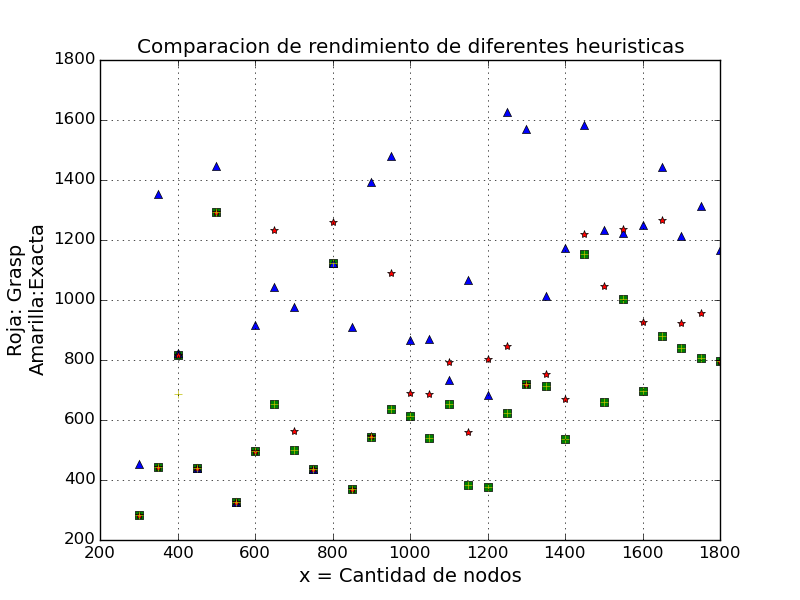
\includegraphics[scale=0.7]{experimentos/performance-optimalidad-lineales-beta_n_over_128/comparacion_optimalidad.png}
\end{center}

%--------------------------------------------------------------------------------------

\subsubsection{Grafos aleatorios de intermedia densidad de aristas}
\textbf{Parametros del experimento:}
\begin{itemize}
	\item Cantidad de tests realizados: 255
	\item Cantidad minima de nodos: 100
	\item Cantidad maxima de nodos: 600
	\item Rango peso $w_1$: [0..250]
	\item Rango peso $w_2$: [0..400]
	\item Cota de $w_1$: 200
	\item Cantidad minima de aristas: $ n * \sqrt n$
	\item Cantidad maxima de aristas: $ 5 * n * \sqrt n$
\end{itemize}

\vspace{1cm}

\textbf{Resultados del analisis (Golosa):}
\begin{lstlisting}[frame=single]	
	Tiempo promedio microsegundos heuristica: 2700.713
	Tiempo promedio microsegundos exacto: 6803.960
	Heuristica da la solucion optima: 86.666% de los casos
	Lejania promedio de la heuristica a la solucion optima: 2.590%
	Desv. estandar de la lejania entre las soluciones: 9.77461
	Minima lejania entre bqlocal y exacta: 0
	Maxima lejania entre bqlocal y exacta: 79.000%
\end{lstlisting}

\textbf{Resultados del analisis (Busqueda local):}
\begin{lstlisting}[frame=single]	
	Tiempo promedio microsegundos heuristica: 529.705
	Tiempo promedio microsegundos exacto: 6803.960
	Heuristica da la solucion optima: 10.588% de los casos
	Lejania promedio de la heuristica a la solucion optima: 726.246%
	Desv. estandar de la lejania entre las soluciones: 904.16
	Minima lejania entre bqlocal y exacta: 0
	Maxima lejania entre bqlocal y exacta: 5900.000%
\end{lstlisting}

\vspace{2cm}

\begin{center}	
	\textbf{Distribucion de los resultados}\\
	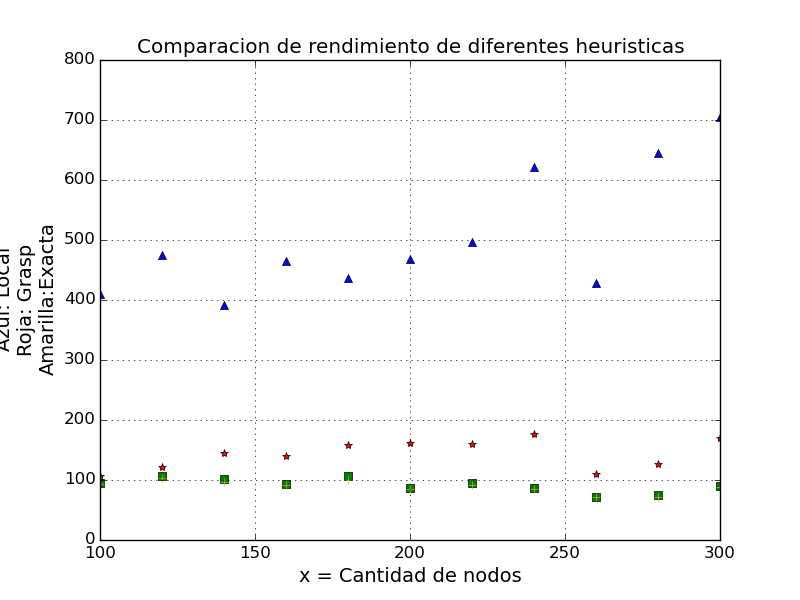
\includegraphics[scale=0.7]{experimentos/performance-optimalidad-intermedios/comparacion_optimalidad.png}
\end{center}

%--------------------------------------------------------------------------------------

\subsubsection{Grafos aleatorios de alta densidad de aristas}
\textbf{Parametros del experimento:}
\begin{itemize}
	\item Cantidad de grafos analizados: 53
	\item Cantidad minima de nodos: 10
	\item Cantidad maxima de nodos: 280
	\item Rango peso $w_1$: [0..250]
	\item Rango peso $w_2$: [0..400]
	\item Cota de $w_1$: 200
	\item Cantidad minima de aristas: $\frac{n * (n-1)}{3}$
	\item Cantidad maxima de aristas: $\frac{n * (n-1)}{2}$
\end{itemize}

\vspace{1cm}

\textbf{Resultados del analisis (Golosa):}
\begin{lstlisting}[frame=single]	
	Tiempo promedio microsegundos heuristica: 4569.584
	Tiempo promedio microsegundos exacto: 19571.283
	Heuristica da la solucion optima: 83.018% de los casos
	Lejania promedio de la heuristica a la solucion optima: 4.990%
	Desv. estandar de la lejania entre las soluciones: 18.1754
	Minima lejania entre bqlocal y exacta: 0
	Maxima lejania entre bqlocal y exacta: 110.300%
\end{lstlisting}

\textbf{Resultados del analisis (Busqueda local):}
\begin{lstlisting}[frame=single]	
	Tiempo promedio microsegundos heuristica: 550.485
	Tiempo promedio microsegundos exacto: 19571.283
	Heuristica da la solucion optima: 13.207% de los casos
	Lejania promedio de la heuristica a la solucion optima: 1042.275%
	Desv. estandar de la lejania entre las soluciones: 1153.29
	Minima lejania entre bqlocal y exacta: 0
	Maxima lejania entre bqlocal y exacta: 4473.000%
\end{lstlisting}

\vspace{2cm}

\begin{center}	
	\textbf{Distribucion de los resultados}\\
	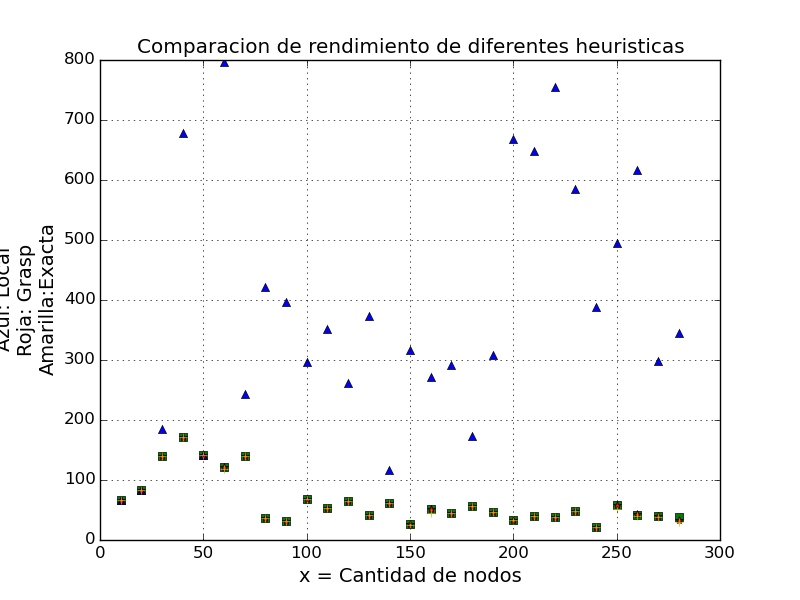
\includegraphics[scale=0.7]{experimentos/performance-optimalidad-cliques_beta_n_over_128/comparacion_optimalidad.png}
\end{center}


\textbf{Conclusion: } Ahora analizaremos como se comportan los algoritmos heuristicos(goloso y busqueda local) respecto a los distintos conjuntos de tests y sus resultados.\\

\vspace{0.75cm}
\textbf{Algoritmo Goloso para grafos de baja densidad:}\\
Vemos que el algoritmo goloso tiene optimalidad cercana al 100\%, aqui dio 98.6\% y en la secci\'on propia del algoritmo goloso dio 100\% cuando se trata de grafos con densidad lineal de aristas, en caso de no dar el optimo, tiene un 0.261\% con una desviacion estandar del 2\% de lejan\'ia respecto a la soluci\'on \'optima. Como contraparte, el tiempo de ejecuci\'on es sutilmente superior al del algoritmo exacto(con 4 podas), seguramente(como se puede apreciar en la secci\'on de rendimiento del algoritmo exacto) para grafos con mayor cantidad de nodos, el tiempo de ejecuci\'on del algoritmo exacto se dispare. Consideramos que el algoritmo goloso es una muy buena opcion si se trata de aproximar soluciones optimas para grafos con densidad lineal con una cantidad de nodos considerablemente alta que produzca que el algoritmo exacto no sea viable.\\

\vspace{0.5cm}

\textbf{Algoritmo Goloso para grafos de densidad intermedia:}\\
Para instancias de grafos con densidades intermedias de aristas, podemos ver como baja levemente el nivel de optimalidad a 86\% de aciertos respecto a la soluci\'on exacta. Tambien se incrementaron a  2.59\% la lejan\'ia promedio y a 9.7\% la desviacion estandar de la lejan\'ia. Sin embargo, sigue siendo una muy buena heur\'istica, porque en este caso si, puede apreciarse que el algoritmo exacto tarda un 250\% mas de tiempo en promedio para llegar a la soluci\'on. Teniendo en cuenta que la cantidad de nodos de los grafos generados va disminuyendo a medidad que aumentamos la densidad(por cuestiones pr\'acticas de realizar los tests en el hardware disponible), observamos que para densidades mas altas de aristas en los grafos testeados empieza a ser una muy buena alternativa la soluci\'on golosa, siempre y cuando el contexto de aplicaci\'on acepte los estimadores de lejan\'ia al optimo.

\vspace{0.5cm}

\textbf{Algoritmo Goloso para grafos de alta densidad:}\\
Finalmente, para el caso mas complicado para el algoritmo exacto(recordemos que en la complejidad, el grado de los nodos es la cantidad de llamadas recursivas que realiza y si la densidad es alta el grado promedio va a ser alto dada la distribucion uniforme de las aristas sobre el grafo), la soluci\'on golosa disminuye muy levemente la efectividad con respecto al caso anterior, tiene un 83\% de aciertos a la soluci\'on \'optima, asimismo aumentan los estimadores de lejan\'ia, en promedio a un 4.99\% con una desviaci\'on de 18.17\%. Respecto al tiempo de ejecuci\'on, el algoritmo exacto tarda en promedio 4.28 veces mas de tiempo para obtener la soluci\'on exacta. Para ser el caso mas dificil de los casos de prueba que consideramos, pensamos que los resultados son muy buenos para las aplicaciones pr\'acticas.

\vspace{0.5cm}

\textbf{Algoritmo de Busqueda local para grafos de baja densidad:}\\
Respecto a la heuristica de busqueda local, observamos un 30\% de efectividad, con una lejan\'ia promedio de 87.62\% y una desv. estandar en la lejan\'ia al optimo de 118.5\%, consideramos que 30\% es un numero muy bajo y junto a los indicadores de lejan\'ia, si nos interesa realmente una solucion cercana a la \'optima no elegiriamos esta heur\'istica(al menos no con dijkstra sobre $w_1$ como soluci\'on inicial. Ver Experimentacion de la solucion inicial en la secci\'on busqueda local). Como contraparte, toma aproximadamente la mitad de tiempo que el algoritmo exacto(recordemos que la medicion es por iteracion y para grafos lineales hay 1 iteracion promedio.), no consideramos que sea un buen tradeoff, la mitad del tiempo de ejecuci\'on para esta calidad de soluciones.\\

\vspace{0.5cm}

\textbf{Algoritmo de Busqueda local para grafos de densidad intermedia:}\\
A medida que vamos aumentando la densidad de los grafos, la b\'usqueda local deber\'ia poder mejorar mas la soluci\'on, de hecho cuando analizamos la variaci\'on de la soluci\'on a medida que avanzan las iteraciones, el mejor caso era donde la densidad era m\'axima, lo que atribuiamos a una vecindad de mayor cardinal, pero cuando comparamos optimalidad promedio de la heur\'istica, nos da un numero baj\'isimo, 10\% de aciertos a la soluci\'on optima, con un promedio y dispersi\'on de lejan\'ia enormes. Atribuimos este bajo rendimiento a la soluci\'on inicial provista realizando dijkstra sobre $w_1$, mas adelante cuando analicemos GRASP, para ciertos valores del par\'ametro beta(bajos, para que se acerque la soluci\'on randomizada a la heur\'istica golosa pura), los experimentos representar\'an una b\'usqueda local alimentada inicialmente por un algoritmo de mayor optimalidad. Dado que la cantidad promedio de iteraciones para densidades intermedias nos dio cercano a 4 iteraciones, el tiempo de ejecuci\'on(por iteracion) multiplicado por 4, nos da como resultado que el algoritmo de b\'usqueda local tarda un tercio del tiempo que el algoritmo exacto, nuevamente, no consideramos que sea un tradeoff aceptable dada la calidad de las soluciones.

\vspace{0.5cm}

\textbf{Algoritmo de Busqueda local para grafos de alta densidad:}\\
Este caso es casi id\'entico al anterior con respecto a la optimalidad de las soluciones, tal vez un poco peor, pero despreciable, lo \'unico que vari\'o considerablemente fue el tiempo de ejecucion del algoritmo exacto a 19571 microsegundos y la cantidad de iteraciones promedio de la b\'usqueda local a 5 iteraciones promedio con un tiempo por iteracion de 550 microsegundos. Veamos entonces que el algoritmo de b\'usqueda local se ejecuta aproximadamente 7 veces mas rapido que el algoritmo exacto. Las conclusiones son las mismas que en el caso de densidad intermedia, no consideramos que sea un buen tradeoff dado el \texttt{baj\'isimo} numero de aciertos a la soluci\'on optima y la enorme lejan\'ia al optimo.

\vspace{0.5cm}

Como conclusi\'on de b\'usqueda local consideramos que depende mucho de la soluci\'on inicial la calidad final de las soluciones obtenidas(nuevamente, ver seccion de variacion de soluciones iniciales en seccion busqueda local). Utilizar\'iamos un esquema de b\'usqueda local para refinar soluciones relativamente buenas obtenidas con algun otro m\'etodo inicial.

\vspace{0.5cm}

\subsubsection{Gr\'aficos de distribucion de las soluciones}
\vspace{0.5cm}
\textbf{Distribuci\'on de soluciones para grafos de alta densidad:}\\
Podemos observar que las soluci\'ones de b\'usqueda local siempre estan lejos del \'optimo indicado por un + amarillo en el eje Y. Con respecto a GRASP, algoritmo goloso y algoritmo exacto se encuentran casi superpuestos, salvo casos particulares.

\vspace{0.5cm}
\textbf{Distribuci\'on de soluciones para grafos de densidad intermedia:}\\
Se observa que los valores de las soluciones provistos por busqueda local estan sutilmente mas cerca de los demas algoritmos, igual siguen estando relativamente lejos, respecto a las otras heuristicas(Golosa y GRASP) comienzan a verse su "despegue" de la soluci\'on \'optima, mas que nada en la metaheuristica GRASP.

\vspace{0.5cm}
\textbf{Distribuci\'on de soluciones para grafos de baja densidad:}\\
Finalmente aqui observamos que la soluci\'on de busqueda local sigue "lejos" del \'optimo. Asimismo, GRASP tampoco provee la soluci\'on \'optima ni una \texttt{muy cercana}, como si lo hace la heur\'istica golosa con su casi perfecto indice de aciertos respecto al algoritmo exacto.

\subsection{Experimentacion pura entre heuristicas}
En esta secci\'on experimentaremos para varios conjuntos aleatorios de grafos de diferentes densidades con las heur\'isticas implementadas,sin tener en cuenta la soluci\'on exacta, para poder realizar experimentos con una mayor cantidad de nodos y aristas en las instancias. Dados los resultados, analizaremos de las 3 heur\'isticas implementadas cual obtiene en promedio y con que desviacion estandar, las soluciones con peso $w_2$ menor, y de esta forma, mas cercanas a la exacta.\\

Esto se realizara, para cada ejecucion de las 3 heuristicas, incrementando un contador en la que corresponda si su peso $w_2$ es minimo, al final tendremos, para cada heuristica, cuantas veces dio la minima solucion, y la cantidad total de instancias testeadas, con estos datos podremos realizar los analisis estadisticos.

poner al menos 15000 nodos, sino no tiene sentido(by guido)